\chapter{The "Stealth" Mission: "Assassination"}

\begin{wrapfigure}{O}{\figwidth}
	\begin{center}
		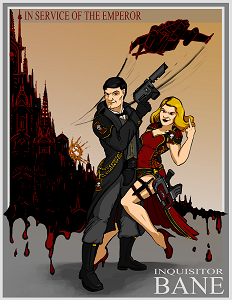
\includegraphics[width=\figwidth]{pics/19/1.png}
	\end{center}
\end{wrapfigure}
So no shit, there we were, standing slackjawed in the rubble of a Crime Lord's private museum, watching the Sorceress we'd just chased through the whole damn mansion making out with BANE FUCKING JOHNS as their gunship flew off into the sunset. 
After a few seconds of disgusted silence, Doc and Sarge cleared their weapons and made a spirited attempt to interrupt the pair's romantic moment. 
None of their shots came even remotely close. 


Down on the floor Tink and Twitch stopped clutching at their respective injuries as they registered the familiar, if a bit deeper than usual, sound of someone overcharging a plasma weapon on the floor above. 
Tink flipped through his comm channels and shouted a futile warning while Twitch yanked a catatonic Nubby into cover a split second before a bright blue explosion collapsed a large section of the ceiling. 
As the rest of us coughed and dug our way out of the rubble, Tink limped his way up the pile of rubble, poked his head out of the smoldering crater, and informed what was left of the other Inquisitorial team that he'd told them so.

\greentext{>The All Guardsmen Party and the "Stealth" Mission: Part 3}

\greentext{>The Return of Bane Johns}


\begin{wrapfigure}{O}{\figwidth}
	\begin{center}
		
\includegraphics[width=\figwidth]{pics/19/2.png}
	\end{center}
\end{wrapfigure}
Fortunately for our mouthy techie, nobody upstairs was in any condition to beat the shit out of him. 
In fact the only one of them that even seemed aware of our arrival was the Fringe-Worlder, who waved at us with the bloody stump of his right arm and asked how "y'all's" part of the mission was going. 
Sarge managed to convey an entire after-action report's worth of disgust and annoyance with a single grunt, which got a weak laugh from the man and a disapproving look from Doc as he tourniqueted the bleeding limb.

While Doc began triaging what was left with the other team (deciding to start with their Interrogator, whose power armor had somehow failed to stop a dozen autopistol rounds), Sarge's attention was caught by a large figure in blackened, smoking Sororitas power armor struggling out of a hole in the wall. 
The Big Sister stumbled over to the windows and tossed the half-slagged remains of a plasma cannon out of them, yanked her equally ruined helmet off and began screaming a string of decidedly un-sisterly Vostroyan curses at the distant gunship. 
Sarge blinked as he finally recognized the face and voice as belonging to Ivana Krushyu, former minion of the traitorous Lord General Omurov, and one of Bane Johns numerous girlfriends before he'd been hauled off by the Inquisition. 
Sarge, no longer feeling capable of surprise, just let out disgusted sigh at the universe's perverse sense of humor, and asked the valkyrion woman if she had any injuries that needed treatment. 
She stared at him for a second, and then dropped to her knees screaming and clutching at her head.

\begin{wrapfigure}{O}{\figwidth}
	\begin{center}
		
\includegraphics[width=\figwidth]{pics/19/3.png}
	\end{center}
\end{wrapfigure}
The last two members of the other team that we could find weren't doing noticeably better than Ivana. 
Tink found what was left of their tech-priest in a crater full of blood, lubricant, and assorted servitor bits, and after a bit of highly scientific stick-poking declared the cogboy to be "super DUPER dead". 
The tech-priest in question took offense at this, loudly complaining that "you take one nap in a pool of your own bodily fluids and people start declaring you all sorts of things". 
He informed Tink that unlike SOME people he could operate just fine without his appendages, and in apocalyptic, low power environments of as few as 1.1 volts too, thank you very much. 
If someone would be so kind as to dig him out, top up his internal battery, and drag him to a servitor workshop he'd arrange for Tink to try being limbless torso and see how alive HE looked. 
Tink was understandably a bit hesitant about helping the cogboy, but was informed that "he's a bit of a dick" wasn't a valid excuse for leaving an ally to bleed out.

The Ganger was in better shape physically, but mentally she definitely a bit out of it. 
She just kept staring out the window, seemingly unaware of our arrival, or the fact that she was sitting on the remains of what appeared to be one of our Interrogator's murder-dogs. 
Twitch, interpreting this shockiness as a sign of daemonic possession (as opposed to, you know, SHOCK), threw a vial of holy water at her, which at least brought her attention back to the general orbital vicinity, if not all the way down to earth as it were. 
Despite Twitch's insistence that she wasn't as angry as she should've been, and was probably harboring a gene-stealer parasite or something, the dampened Ganger was allowed to keep her various weapons (we didn't have the spare bag space for them anyway) and was tasked with getting the wounded Fringe-Worlder up and moving.

\begin{wrapfigure}{O}{\figwidth}
	\begin{center}
		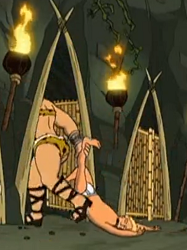
\includegraphics[width=\figwidth]{pics/19/4.png}
	\end{center}
\end{wrapfigure}
Back across the room, Ivana finally transitioned from tortured screaming to a mix of hysterical giggling and tears. 
Not being emotionally equipped to deal with crying women in general, much less one a head taller and twice as burly as himself, Sarge decided this probably meant she was uninjured and beat a rather cowardly retreat. 
He'd only got a few steps before the crying abruptly stopped, and a large power-armored hand grabbed him by the shoulder. 
A deep, scarily-focused voice informed him that he was Needed. 
For A Thing. 
Right Now. 
Sarge made a small whimpering noise.

To our not-so-fearless leader's relief, he was only dragged over to where Doc was failing to treat the other team's Interrogator's numerous autopistol wounds. 
Completely ignoring the medic and his work, Ivana saluted her half-dead Interrogator and in a parade-ground voice announced that Interrogator Sargent was formally requesting to transfer to their team. 
The requestee's confused "I am?" earned him a glare, a possibly broken shin, and a threatening "Yes, you are"; 
Sarge wisely decided just to go with it and hope that it wouldn't all end in some sort of Inquisitorial tribunal for gross misconduct.

In a complete farce of Inquisitorial procedure, with Ivana creatively interpreting the pained gurgles of her superior officer, Sarge was inducted into the retinue of Inquisitor what's-his-name. 
Then, since said Inquisitor had last been seen being sucked screaming into a hole in the warp after trying to use his psyker powers on Bane, and his Interrogator had apparently kicked the bucket mid-ceremony, Sarge was appointed acting Inquisitor, handed a shiny Ordo Hereticus rosette, and put in charge of the team. 
At least, that's what Ivana said was going on; 
the Fringe-Worlder accused her of being crazier than a bag of something or other, but recommended we just play along and keep the rosette away from her until we'd gotten out of there. 
We quietly agreed with him.

\begin{wrapfigure}{O}{\figwidth}
	\begin{center}
		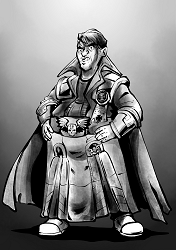
\includegraphics[width=\figwidth]{pics/19/5.png}
	\end{center}
\end{wrapfigure}
The other team having been collected (literally in the tech-priest's case) Doc raised the question of where our teammates were and why we'd gone and entire five minutes without Sciscitat yelling at us. 
Tink  answered the latter by poking at his combead for a second before hastily deactivating it and informing everyone that A: 
plasma interference or space fairies or something had fouled our comms so they all needed to be restarted and B: 
the Inquisitor REALLY wanted to talk to Sarge.

Given the fact that we were in the middle of both a Crime Lord's mansion and a large scale assault by the Planetary Secret Police, Sarge kept his report to the half-furious, half-frantic Sciscitat brief, leaving out the hard to explain details about Ivana and Bane and such. 
The Inquisitor stuck to the basics as well, settling for just a few darkly sarcastic comments when he learned about the Inquisitor's death and the Sorceress' escape with the evil box thing. 
The mission being well and truly scrubbed, we were given the order to pull out. 


The original plan called for extracting via the parking garage, but we were quick to point out that, since the Secret Police had launched their attack from that way, we probably wouldn't be able to reach those fancy getaway cars. 
And even if we could get to them, they'd likely been damaged in the fighting or something; 
it was probably best to not even try recovering them. 
Sciscitat seemed suspicious, but grudgingly guided us on a path to recover our surviving teammates and exit via the route which the second team had used to get in.

\begin{wrapfigure}{O}{\figwidth}
	\begin{center}
		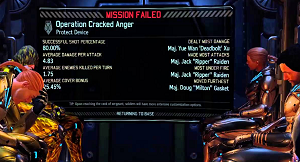
\includegraphics[width=\figwidth]{pics/19/6.png}
	\end{center}
\end{wrapfigure}
Nubby was picked up from where he'd been left moping heartbrokenly around the wrecked art museum, and was attached to the shell-shocked Ganger, who just nodded along vacantly with his self-pitying monologue. 
From there we made our way back along the trail of destruction Bane had left in his wake, collecting what was left of our teammates who'd tried to attack the two decoy sorceresses and ran afoul of their "bodyguard". 
Of the four of them:
\greentext{>The Deathcult Assassin was dead: he tried to knife-fight Bane.}

\greentext{>Face was still breathing but completely catatonic and bleeding from the eyes. Doc put it down as "warp bullshit" and said he'd probably be fine. Or he'd turn into a deamonhost. One or the other.}

\greentext{>The Cleric had been shot. Again.}

\greentext{>One more of our Interrogator's cybernetic murder-dogs was definitely dead, and another had had last been seen sailing out a window, but the woman herself had made it through unscathed thanks her decision to chase the decoys instead of Bane.}


Thankfully, the Cleric was still capable of walking, so only Face had to be carried, and the Interrogator was actually being cooperative for a change. 
We'd expected yet another argument about who was in charge, or at least some incessant whining about her dead pets, but she just quietly fell into line at the back of the group and even followed Sarge's orders. 
We were incredibly grateful for this given the difficulty of sneaking our whole ragged little patrol passed all the Goons and Secret Police. 
Twitch declared it to be incredibly suspicious though, and Ivana constantly seemed to be watching the Interrogator when we weren't on the move too.

\begin{wrapfigure}{O}{\figwidth}
	\begin{center}
		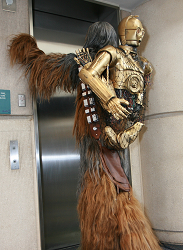
\includegraphics[width=\figwidth]{pics/19/7.png}
	\end{center}
\end{wrapfigure}
It took three hours and a whole lot of stairs to make it down to where the Crime Lord's little sub-spire connected to the hive, and then back up to a vehicle-accessible area that wasn't crawling with Planetary Secret Police. 
The only real moment of interest was a brief firefight with the bodyguards of some noble fleeing the giant charlie-foxtrot above, at the end of which Ivana's half-slagged power armor finally gave up the ghost. 
The Sororitas armor was unceremoniously ditched in a closet. 
The torso-fied tech-priest in Tink's backpack loudly complained that he'd just fixed the stuff after SOME ASSHOLE WITH A PLASMA GUN shot up its power unit. 
He then directed said asshole in the looting of "the good bits" of the discarded armor, which might be useful in fixing some of the long list of obvious amateur mistakes SOMEONE had made on their plasma weapon. 
Tink asked if someone else could carry the tech-priest, but was informed they made a cute couple.

Also on the note of Ivana, the disarmed Fringe-Worlder pulled some of us aside for a few words, to "explain her". 
In short, she was crazy. 
Like actually certifiably. 
His boss had snagged her up for no other reason than to spite Oak for trying to recruit her on Hereticus time, which explained a lot, and she'd subsequently undergone some psyker-assisted "reeducation", which explained even more. 
His point was that Ivana was sweeter than a something full of somethings, but even if we'd served with her before (as he was s'pectin') it wouldn't be a good idea to bring up her past. 
Or her fixation on Inquisitorial authority. 
Or whether or not she was actually a Sister of Battle. 
Or certain varieties of mixed drinks. 
Best if we didn't talk to her at all really. 
Especially given that the woman in question had twisted one of those bodyguards' head off like a bottle-cap, and was alternating between glaring at our other female companions and eying Sarge with a downright disquieting level of intensity.

\begin{wrapfigure}{O}{\figwidth}
	\begin{center}
		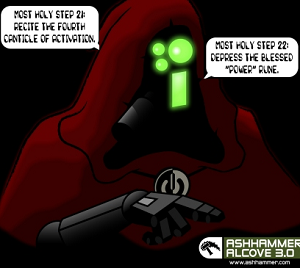
\includegraphics[width=\figwidth]{pics/19/8.png}
	\end{center}
\end{wrapfigure}
The Scan Van was waiting for us at our eventual exit along with the definitely-not-full-of-orks truck, which was being driven by two heavily armed men we didn't recognize, but the Fringe-Worlder vouched for. 
We decided these strange men, who'd almost certainly been tasked with killing our team in the event that we doublecrossed their now-dead Inquisitor, were just the folks to take our large collection of wounded teammates (with one specific exception) off for medical treatment by their team's actual real doctor. 
Sciscitat probably didn't agree with that judgement, but we were suffering some mysterious comm interference.

Once the truck had pulled out, we directed our attention to the Scan Van, or more specifically, its driver. 
During the hike out, the question of what to do about a certain problematic tech-priest had been raised, and the other priest had been tapped for some expert advice in dealing with his die-hard orthodox counterpart. 
This wasn't intentional, we just forgot he was in Tink's pack and could totally hear us. 
In any case, he cheerfully suggested turning our cogboy off and on again. 
With our lasguns. 
Admittedly the "on again" part would be tricky, but he thought it was still worth a shot. 
We decided we liked the Torso-priest.

\begin{wrapfigure}{O}{\figwidth}
	\begin{center}
		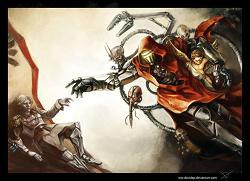
\includegraphics[width=\figwidth]{pics/19/9.png}
	\end{center}
\end{wrapfigure}
Doc entered the Scan Van via the rear door, triggering at attack of horrible nausea in the exhausted psyker occupying it. 
Seeing the man's discomfort, Doc graciously administered a dose of anti-nausea medication, which had the completely accidental side-effect of knocking Snitch out cold. 
In the front of the van, Lexmechanic Thomas de Torque's attempts to localise the signal jamming his vox connection to the Inquisitor were interrupted by someone knocking on the passenger door. 
He was still trying to explain to the dolt outside that the door was locked and would remain that way, when the window behind him exploded in a shower of safety glass and a pair of beefy arms seized him by the neck. 
As the tech-priest's datafeeds were ripped from their sockets and he was dragged kicking and screaming out the broken window, he reflected on the wisdom of antagonizing a bunch of people who viewed violence as more of a first resort. 
The last thing Thomas heard, aside from all the las and plasma fire, was a muffled mechanical voice calling "dibs" on his limbs. 
He hoped it was the Omnissiah.

Sciscitat was less than pleased to find out his tech-priest had been replaced with a new lighter-weight model. 
For some reason he didn't seem willing to believe Sarge's report of a last-second sneak attack on the scan-van (even with all the super-realistic combat sound effects being supplied in the background by Twitch and a slightly cheered-up Nubby). 
That said, the Inquisitor didn't really seem angry about the brutal murder of a trusted subordinate, so much as annoyed at the great personal inconvenience it would cause him, whining about how much of his valuable time it would take to bring the new cogboy up to speed and so on. 
In retrospect, why we'd expected any other response was a mystery.

So yeah, Sciscitat took the news pretty well... 
right up until Sarge sort of accidentally mentioned Bane and Angelica.

By name.

And rank.

\begin{wrapfigure}{O}{\figwidth}
	\begin{center}
		
\includegraphics[width=\figwidth]{pics/19/10.png}
	\end{center}
\end{wrapfigure}
Doc and Twitch tackled Sarge and took away his combead, but the enraged screaming had already started by that point so we just went with Plan B and Tink reactivated the jammer. 
Our new tech-priest informed us that we were idiots delaying the inevitable; 
Doc reminded him that we were guardsmen.

The beauty of Plan B was that, between the limb-attachment (a process which involved a lot of sarcasm and backseat surgery-ing from the patient) and the inter-hive traffic delays caused by some big dust storm thing and all the Arbite patrols, we got twelve hours of napping in before the inevitable shit-show of the debriefing. 
This was a very good thing, because the revelation that not just one, but BOTH of the Conspiracy agents were our ex-bosses didn't go over well with the Inquisitor. 
Or anyone else for that matter, especially the two new guys from the other team, who turned out to be REAL Inquisitorial Stormtroopers and were therefore already a bit ill-disposed towards us. 
It was only Sciscitat's repeated assurances that we were too stupid to have actually planned everything that kept us from being branded traitors on the spot; 
Sarge thanked him for his support. 


That set the tone for the rest of the debrief, though admittedly it could've been worse: 
for instance the tech-priest might've still been alive (that thought alone was enough to keep our morale up through the whole thing). 
Also, Snitch was too wiped out to do much of his usual fact checking, so that was nice, and Face spent most of the meeting lying in a corner muttering "wiggle your big toe" to himself. 
The Interrogator was doing a little better (see: 
bitchy), but some sort of feud with Ivana drew most of her fire off us, so it was mostly just Sciscitat, the Cleric, and the two Stormtroopers picking everything apart and finding varying degrees of fault with our every action.

\begin{wrapfigure}{O}{\figwidth}
	\begin{center}
		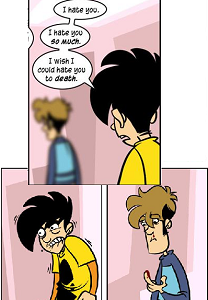
\includegraphics[width=\figwidth]{pics/19/11.png}
	\end{center}
\end{wrapfigure}
Despite a strong temptation to throw Nubby under the proverbial bus, we responded to the nitpicking with a mixture of apathy, antipathy, and (in Twitch's case) sociopathy. 
As far as we were concerned the reappearance of our old bosses had changed the nature of our mission, and we no longer had time for these silly little games. 
Eventually Sciscitat and his minions took the hint and moved on to more productive subjects. 
It was amusing to watch as they realized that the only people with actual intel on Bane and Angelica were the ones they'd spent the last two hours badmouthing, not that it stopped them from constantly interrupting our report. 


To say that the stories of our past missions with the two ex-Interrogators was met with a little skepticism doesn't quite cover it. 
"You're making this up", "Bullshit", and "If that actually happened, then I'm an Ork in dress. 
Why is he looking at me like that?" sums it up a bit better. 
Things started to go downhill pretty quickly until, to our considerable surprise, Sciscitat stepped in and told everyone else to shut up and actually listen to us. 
Unfortunately, any gratitude we felt for this intervention evaporated where we got to our patented "DTU Strategy", and the Inquisitor pointed out that this was probably why the Secret Police had been rounding up every untouchable on the planet... 


The real kicker was finding out that EVERYONE, including Ivana who LITERALLY HAD BRAIN DAMAGE, had been told except for us. 
We dearly missed the days when Sciscitat attended meetings in person, because then we could've shot him like he deserved.

\begin{wrapfigure}{O}{\figwidth}
	\begin{center}
		
\includegraphics[width=\figwidth]{pics/19/12.png}
	\end{center}
\end{wrapfigure}
Anyway, despite her supposed memory problems, Ivana also chimed in to claim Bane had some sort of subtle mind control powers, and that these had already been used on the Ganger (which explained why she wasn't present). 
Ivana's teammates backed her up on this, but were a bit less supportive when she went on to accuse our Interrogator of being "compromised" as well. 
Twitch was totally on board though, and excitedly began listing all the "suspicious" ways our nominal superior had been acting. 
He probably should have stuck to just the post-mission stuff though, the amazingly detailed log of her personal hygiene habits and what fiendish plots they might be hiding didn't really help his argument. 


To Sciscitat's credit he took Ivana's (if not Twitch's) accusation seriously enough to wake Snitch up and have the psyker take a few pokes and his Interrogator's brain despite some pretty strong protests on her part. 
Unfortunately, he had a bit less patience when Snitch declared her to be clean of outside influence and Ivana still persisted. 
The term "crazy bitch" was used a few times. 
Eventually, between her teammates and Sarge's own reassurances, Ivana was convinced to settle for a vague promise to keep an eye on our Interrogator.

Since things had pretty much stalled by this point, Sarge decided it was time to raise the question of just what in the Emperor's name we were going to do about Bane and Angelica. 
The Fringe-Worlder earned our undying approval by immediately suggesting nuking them from orbit, but this was shot down by Sciscitat on the grounds that it would destroy the Artifacts in their possession. 
Twitch grimly added that he wouldn't believe Bane was dead unless he personally saw the body. 
Even if we called in a full Exterminatus, some scavengers would probably just find him a few weeks later in a stasis-equipped refrigerator up in orbit or something. 
Doc hushed him, and Sarge took the floor to present Plan C.

\begin{wrapfigure}{O}{\figwidth}
	\begin{center}
		
\includegraphics[width=\figwidth]{pics/19/13.png}
	\end{center}
\end{wrapfigure}
Plan C (A and B being the aforementioned Untouchable and Nuke It From Orbit) consisted of separating our two ex-bosses through some vaguely defined trickery, dealing with Angelica using "literally all of the explosives", and just throwing disposable bodies at Bane until he got tired from killing them. 
As plans went it was admittedly a bit of a work in progress, but we felt it set a good general theme to start with.

The Torso-priest raised the question of whether Bane was or wasn't a daemonhost and how that would affect tiring him out. 
Tink pointed out that A: 
with Bane, how could you tell? 
And B: 
either way his powers were warpy, and if you keep using warp powers for long enough you'll either explode or turn into a daemon; 
it's just how magic works. 
Nobody argued either point, though Tink did get some pushback when he went on to suggest that we could accelerate the process by adding a few disposable psykers to the mix. 
The argument was progressing nicely and was on the edge of turning into a real plan, when Sciscitat broke in to inform everyone that we wouldn't be doing that, ANY of that. 


The Inquisitor explained to us slow people that our mission was to get the artifacts, NOT kill rogue Inquisition agents. 
Everyone present stared at him with the incredulity that statement definitely warranted until Doc bit the bullet and asked how he intended to get anything done without at the very least killing Bane first. 
Sciscitat just rolled his eyes and explained that the way you dealt with tactically superior enemy was to plan AROUND their strengths and outmaneuver them on strategic level. 
It was okay, he didn't expect us to understand. 


To our disgust, several of the other, theoretically sane, people present actually nodded along with the Inquisitor's bullshit. 
 Sarge took a deep breath, summoned up every ounce of his half-assed diplomatic training, and attempted to convince Scicitat that he wasn't quite grasping the scope of Bane's powers. 
He was not successful.

\begin{wrapfigure}{O}{\figwidth}
	\begin{center}
		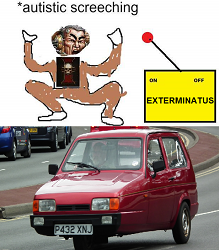
\includegraphics[width=\figwidth]{pics/19/14.png}
	\end{center}
\end{wrapfigure}
We belatedly realised that, despite not being physically involved in the recent mess, the Inquisitor hadn't been having the best day. 
When Sarge tried to explain how terrible his idea was and how dead we would all get attempting it, some sort of dam burst inside the man. 
It was... 
well, you couldn't call it "impressive" exactly, what with his stature and the fact that he was only a hologram, but it was definitely a bit surprising. 
Like being savaged by a fat little dog. 
A yappy one. 
It would've been hilarious if he wasn't our direct superior.

Sciscitat's little tantrum ended with him declaring us banned from all meetings, and ordering us out to do some "things, very important things, things at least two hives away from here". 
Tink smugly pointed out that it would be a tad tricky, given where we'd left our van parked. 
The Inquisitor almost grinned as he pulled up a hologram of a tiny three-wheeled ground car and informed us that the tech-priest had managed to order us a replacement before his unfortunate demise. 
Certain people around the table snickered; 
Snitch began to inform everyone what we thought of our new ride, but paused at a glare from Sarge, who very pointedly remained in his seat.

After a few seconds of mutual glaring Sciscitat pulled up another hologram, this time of a familiar massive armored figure standing in front of a whole precinct of Arbites. 
Nubby swore and threw one of the several beer bottles he'd emptied over the course of the meeting through it. 
The Inquisitor ignored this, and grimly informed the rest of us that, if we couldn't even follow the simplest orders, he knew a certain rising star in the Arbites who'd probably be willing to trade all sorts of support for information regarding van full of guardsmen. 
We took the hint.

\begin{wrapfigure}{O}{\figwidth}
	\begin{center}
		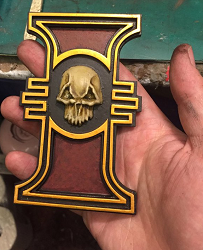
\includegraphics[width=\figwidth]{pics/19/15.png}
	\end{center}
\end{wrapfigure}
It was as we were prying a very drunk Nubby off the floor (we had no idea where he kept pulling the bottles from, Doc just gave up trying to confiscate them after the ninth one and decided it was probably for the better to let the heartbroken trooper drink his sorrows away). 
Anyway, it was as we were picking the little idiot up that *it* happened. 
Threat made, Sciscitat had dropped us from his attention and begun outlining his plan for integrating what was left of the other team into ours. 
Under his Interrogator. 


Ivana leapt to her feet, but instead of the explosion we were expecting, she merely announced that her team couldn't agree to any reassignment without authorization from their Inquisitorial superior. 
This outburst mostly just earned her the same mix of confused and annoyed looks Twitch's remarks usually got; 
except from the Fringe-Worlder, who sighed and pulled his hat down over his face, the Torso-Priest, who was very suddenly at the far end of the room, and Sarge who was too busy staring at Sciscitat's hologram trying to see if it was possible to hate someone to death to notice until Doc kicked him in the shin. 
Sarge suffered a brief moment of panic as he registered the better part of one hundred fifty kilos of woman staring at him like starving dog eyes a poorly guarded bacon sandwich, then finally remembered what he had in his pocket.

The series of changes in our fearless leader's expressions as the situation finally hit him was really something to see, but it had nothing on the reaction around the table when Acting Inquisitor Greg Sargent pulled "his" blood-spattered Ordos Hereticus Rosette out of his pocket, and formally denied Ivana permission to join Sciscitat's team.

\begin{wrapfigure}{O}{\figwidth}
	\begin{center}
		
\includegraphics[width=\figwidth]{pics/19/16.png}
	\end{center}
\end{wrapfigure}
When you're committing something that might technically be considered mutiny, especially against the Inquisition, it's important to keep up your momentum. 
Best to not get bogged down in little things, like the actual meaning of the rules and ordinances you're citing, or whether they even really exist for that matter. 
Which is why the first thing we did after Sarge's announcement was mute Sciscitat's hologram. 
The second was to position Doc as close as possible to Snitch, who quickly turned green and spent the rest of the meeting trying (and eventually failing) to keep his lunch down. 
The playing field nicely leveled, Sarge delivered his pitch.

Now, over the past months we'd given our fearless leader no end of shit for his little diplomacy lessons and their lackluster results, but this is where they finally paid off. 
He might not have had quite the poise or menace of a REAL Inquisitor, and he probably shouldn't have referred to his predecessor as "Inquisitor what's-his-name", but he still managed amazingly well all things considered. 
Sarge explained that we were going to go off and start our own team, just us guardsmen and Ivana, and WE were going to go kill Bane and Angelica. 
Nobody from the other team was required (or even asked) to come with us, they had their own very important mission to complete after all, and it would no doubt be easier accomplish with their two primary opponents dead. 
Of course, we'd still liaise, cooperate, and SHARE CRITICAL INTEL with them just like any other "friendly" Inquisition team would, but they had their objective, we had ours, and that was all there was to it.

I'd like to say we left to mixture of stunned silence and scattered applause, but it was more of a "you won't last ten minutes" atmosphere. 
The moment was spoiled even further a few minutes later when Doc poked his head back in to ask if the Torso-Priest could give us a ride, since there was no way we were ever going to fit Ivana into that three-wheeled thing.

\begin{wrapfigure}{O}{\figwidth}
	\begin{center}
		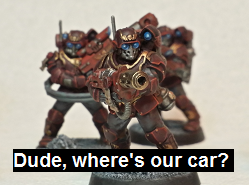
\includegraphics[width=\figwidth]{pics/19/17.png}
	\end{center}
\end{wrapfigure}
Four days later, the "C Team" convened in the briefing room of "Fort Kickass" for the first real planning session of operation "Kill Our Old Bosses". 
The first order of business was to revoking Tink's naming privileges.

Our new base, whatever it was called, was located in the middle levels of the planetary capital: 
Seven Hive. 
We hadn't actually intended to move a third of the way across the planet, it was just that our original plan to simply take over the other team's base met with a bit of opposition. 
Well, not so much "opposition" as "armed resistance", specifically from the two Stormtroopers. 
Sciscitat had apparently flown them out ahead of us, and they didn't seem to agree with us about which of their former bosses assets should pass on to his completely legitimate successor. 
Words, and a few death threats, were exchanged in the doorway before an agreement was finally brokered by the Fringe Worlder. 
We left with a (big) box full of Ivana's stuff, a single dataslate labeled "Person of Interest: 
The Sorceress", and an IOU for "One Inquisitorial Mission Budget". 
Admittedly, not the best Deal we'd ever made, but given our usual negotiator spent the whole time drunkenly sobbing in a corner... 
well, we had to take what we could get.

Honestly, it wasn't like we really NEEDED the budget or intel. 
Those are what we in the Guard refer to as "luxuries", a proper soldier knows how to scrounge. 
For starters, we needed a vehicle we could drive ourselves, and preferably wasn't filled with listening devices piping our every word to our third-worst enemy in the system. 
Fortunately, there were two of them just sitting unattended in that garage. 
Judging by what they yelled after us, the Stormtroopers didn't think their cargo truck and brand new flier had been part of the deal, but we really didn't see how that was our problem.

\begin{wrapfigure}{O}{\figwidth}
	\begin{center}
		
\includegraphics[width=\figwidth]{pics/19/18.png}
	\end{center}
\end{wrapfigure}
That truck served us well over the next few days, the flier, well... 
It'd occurred to us that there was a bit more ground traffic on the planet than was normal, but we'd put that down to local custom or whatever. 
It never occurred to us that there was an actual legitimate reason until Tink reached the edge of Jack Hive and saw how much bigger that little dust storm had gotten since we'd driven through on the way back from the mission. 
I mean, none of us were desert worlders, we'd thought the giant force-shields over all the Hives had been for orbital defense or something... 
What sort of messed up planet has sandstorms that cover whole continents? 
And why would anyone ever build hives on one? 
We asked some of the locals, but all we ever got was some bullshit about planetary ecology and Rogue Traders working in mysterious ways.

Anyway, we'd already decided it'd be for the best if we left Jack Hive, so we wound up just hawking the flier instead of trying to figure out how to transport it via ground or armored shuttle. 
Of course doing this required getting Nubby sobered up and at least nominally functional, which was a project all on its own. 
Doc made liberal use of the various anti-something-or-other pills that'd come with Ivana's stuff. 
They'd been handed over by a pudgy old woman who we assumed was the other team's surgeon, and had come with a detailed administration guide, but Ivana insisted she really didn't need all (or really any) of them, so we had plenty to force down Nubby's throat until the desired result was achieved. 
Doc hadn't exactly approved of this treatment, not that any of that "medical ethics" and "substance dependency" stuff had actually stopped him from administering the pills, he just complained a lot while doing it. 
Sarge promised he'd figure out a better solution, possibly involving an actual licensed therapist, once we got to our new base.

\begin{wrapfigure}{O}{\figwidth}
	\begin{center}
		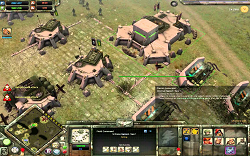
\includegraphics[width=\figwidth]{pics/19/19.png}
	\end{center}
\end{wrapfigure}
Getting to said new base went smoothly enough, all things considered. 
Our exit from Jack Hive was made slightly interesting by a large number of traffic cops and Arbite patrols (suspiciously large in our opinion). 
Fortunately, the low-hive route Nubby's used-flier guy sent us on got us passed most of them, and the one traffic cop that did stop us didn't seem to know what to do when he encountered Ivana in the driver's seat. 
We heard him muttering about transvestite truckers as he stalked back to his bike.

Once on the Inter-Hive it was smooth (if a tad windy) driving to Seven, which was chosen as our destination for the simple reason that it was where the dossier said Angelica and the Secret Police were based. 
Admittedly, that was probably the same exact reason Sciscitat and the other team HADN'T made their bases there, but we felt they were overthinking things a bit. 
The place was a HIVE damnit, they're BIG, even with Bane's bullshittery we highly doubted she'd be able to keep the whole place on lockdown. 
The border though, and the big vehicle inspection checkpoints leading through it, that was a slightly different story; 
fortunately we were Highly Trained Inquisitorial agents.

Now, whatever passed for the Inquisitorial handbook probably has a whole chapter dedicated to  inserting oneself into hostile territory without raising suspicion. 
There's got to be pages and pages about disguises, facial reconstruction, falsified identification documents, black market traffickers, and probably even more on how to covertly make contact with the local authorities. 
We didn't do any of that, instead we drove right up to the lane marked "military", showed the inspector and duty officer a stack of perfectly legitimate (if a bit dog-eared) papers identifying us as Guardsmen of the Generian 99th Medium Infantry, and asked to be billeted while the Administratum sorted out what to do with us.

Very sneaky.

\begin{wrapfigure}{O}{\figwidth}
	\begin{center}
		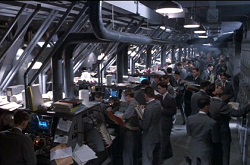
\includegraphics[width=\figwidth]{pics/19/20.png}
	\end{center}
\end{wrapfigure}
We could almost hear the various people who'd (futilely) tried to instill Inquisitorial professionalism into us sighing and rolling their eyes as we were processed through the checkpoint and escorted to the third-largest PDF base in the Hive. 
They weren't guardsmen though, they didn't understand the colossal inefficiency, inflexibility, and general incompetency that was the Departmento Munitorum (well, at least when applied to any problem smaller than planetary invasion). 
There were stories of entire misplaced regiments who'd settled, started families, died of old age, and passed into local legend before their reassignment orders came through. 
At which point they were presumably dug up by their descendents and shipped off to the front, much to the exasperation of whichever Lord General was running the operation, not to mention the poor grunts holding out for reinforcements. 


The point is that we probably had a good year or seven before anyone from Administratum noticed our unexpected resurrection, and while the locals might be a bit more on-the-ball, they were also a lot easier to mislead, confuse, bully, and bribe. 
Add to that we were Real Guardsmen, with the scars and war stories to prove it, and, well... 
By the end of the day we had our very own barracks, with attached motor-pool, plus a stack of chitties for the base mess, several sets of insignialess Haarlockian PDF fatigues, and even an advance on our first week's pay. 
Certain people were in favor of putting in for the years of backpay we theoretically had coming too, and maybe some travel comp if Tink could fabricate the proper documents, but Sarge ruled it was better to quit while we were ahead. 
It wasn't like we really needed the money anyway, between the flier, several miscellaneous items our former teammates hadn't really needed, and a few small shiny objects that'd fallen into Nubby's pockets while we'd been in the Crime Lord's little art museum, we had the budget situation fairly well covered.

\begin{wrapfigure}{O}{\figwidth}
	\begin{center}
		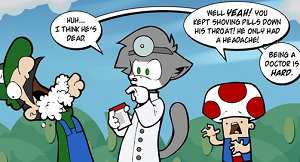
\includegraphics[width=\figwidth]{pics/19/21.png}
	\end{center}
\end{wrapfigure}
On the note of our quartermaster, once we'd settled Doc put his foot down and refused to give Nubby any more Inquisition-strength anti-crazy pills. 
At least until he could find a list of their side effects, not to mention some actual dosage recommendations; 
he hadn't much liked the zombie-ish way the little trooper had been shuffling along the last few days. 
Sarge promised the medic that once Nubby had come fully down, they'd have a heart-to-heart about the whole "girlfriend" thing. 
Unfortunately, the noncom got a bit distracted with all his newfound Inquisitorial duties, and by the time he actually got around to it the little trooper had vanished.

A few hours of frantic searching turned Nubby up in a base-adjacent watering hole, regaling an entire bar full of PDF troopers with a thoroughly classified tale of heartbreak and woe. 
Fortunately for the little idiot's life it was Doc and Twitch who found him, not Sarge, and none of the troopers seemed to actually believe any of his "my hot Inquisitor girlfriend left me for the galaxy's most annoying secret agent" bullshit. 
Doc and Twitch quietly paid his tab and dragged his drunkenly-protesting ass out the door before he violated operational security any further. 
Once back at base, he was tied to a chair, sobered up, and given The Talk.

\begin{wrapfigure}{O}{\figwidth}
	\begin{center}
		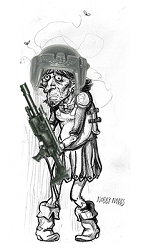
\includegraphics[width=\figwidth]{pics/19/22.png}
	\end{center}
\end{wrapfigure}
This was not your usual The Talk. 
It did start that way, with the typical "she was using you", "you've got to move on", and "it was never really like that", the problem is that that last one isn't supposed to be quite so literal. 
Yes, he did spend a lot of time with her and had been "given" quite a few mementos to remember her by, but those were more grounds for a restraining order than a deep heartfelt a relationship. 
And then there were the weeks of one-sided conversation with her while she was medically paralyzed next to him in the medbay, and the similarly one-sided pen pal relationship afterwards... 
Sarge and Doc both tried, but they had to keep stopping to go and alternatively laugh and swear at the perversity of it all. 


It was draining, it was frustrating. 
Doc was about ready to go back to the pills (and possibly grab a few for himself), and Sarge was considering the merits of locking the idiot up in the brig for the rest of the mission, but eventually they got through to him. 
Except by they, I mean Twitch and Ivana, who shelved the whole "love" issue in favor of focusing on Angelica's newfound relationship with Bane, and to an, um, unexpectedly detailed degree. 
The end result was... 
well... 
acceptable. 
Simmering betrayed rage (at least insofar as Nubby was capable of that emotion), WAS an improvement over drunken, heartbroken sobbing after all. 
Even if it did come along with frequent rants about how nobody could ever compare someone as unquestionably lesser as Bane Johns to such an upstanding individual as Nubby Nubbs, valiant Hero of the Imperium and all around Nice Guy... 


We took what we could get, there was shit to do and people to kill.

\begin{wrapfigure}{O}{\figwidth}
	\begin{center}
		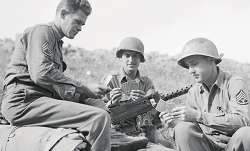
\includegraphics[width=\figwidth]{pics/19/23.png}
	\end{center}
\end{wrapfigure}
First thing first, we needed a plan with less ??? 
in it, and for that we needed Intel. 
Problem was, intelligence gathering wasn't exactly our strong suit, it's what we'd always had all those Adepts for after all. 
Still though, given some of those adepts (not to mention Interrogators and Inquisitors), we figured it couldn't be TOO hard, right?

To start with, Sarge went to have a chat with his PDF counterparts, especially the salty old bastards at the training compound a few levels down-hive from our home base. 
It's a little-known fact outside the Guard, but soldiers are quite possibly the biggest gossips you'll ever find. 
Washerwomen, barmaids, and upper-crust socialites have nothing on a squad of bored troopers on work detail or lounging around their barracks with nothing to do. 
Want to make a juicy secret public knowledge? 
Mention it within earshot of one of those expressionless, easily ignorable gate-guards, and every trooper in regiment will know it by next chow call. 
 It's a widely believed fact that the military grapevine can actually outpace the Astra Telepathica, if the story's good enough that is. 
NCO's are no exception to this rule, in fact they're the ones with the juiciest tidbits, it's just a matter of getting them talking. 
Sarge could do this, easily; 
the real challenge was getting them to shut up again once they got going.

\begin{wrapfigure}{O}{\figwidth}
	\begin{center}
		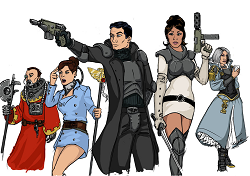
\includegraphics[width=\figwidth]{pics/19/24.png}
	\end{center}
\end{wrapfigure}
Now, it's been said that, the military grapevine can actually outpace the Astra Telepathica. 
If the story's good enough that is, which is where the problem lies for Inquisitorial types. 
Secret heretic cabals, shadowy puppet masters, and secessionist plots don't qualify as "interesting" , at least not according your average grunt. 
If Sarge had gone in there trying to get info on Angelica and her Conspiracy buddies he'd have struck out (well, maybe not if one of them had seen her in person, but even then it wouldn't be her nefarious plots or political maneuvering that they'd be talking about). 
Fortunately though, our other target just so happened to be Bane Johns, self-styled Interplanetary Man of Mystery, and just about the least subtle person this side of the Eye of Terror. 


Sarge didn't even have to try: 
the second story he heard was about someone gunning down an entire underhive street-racing ring for stealing his car, finding out it had actually been towed, and somehow winding up sleeping with the daughter(s) of the hive's Traffic Control Coordinator. 
All while blind drunk. 
The third, sixth, and eight stories were all Bane too, and it didn't take long to find out there was actually a celebrity tabloid dedicated entirely to him. 
It was honestly sort of sad, especially when Sarge realized he'd seen the tabloid on sale weeks ago. 
It definitely raised the question of what the hell Sciscitat and his minions had been doing all this time. 
(I mean, how do you just ignore something like "Gas attack on planetary rare metal reserve! 
Business mogul thrown from private flier! 
Deadly hat attacks! 
Famous aerobatics ace falls in love! 
You'll never guess what these four things have in common!")

\begin{wrapfigure}{O}{\figwidth}
	\begin{center}
		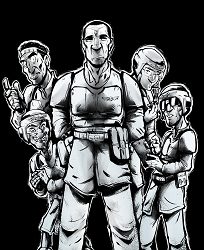
\includegraphics[width=\figwidth]{pics/19/25.png}
	\end{center}
\end{wrapfigure}
It didn't take long for Sarge to pinpoint the general region Bane called home, get in touch with the PDF and hive police forces that patrolled the area, and ask them some pertinent questions. 
By the end of two weeks we knew everything about the man's location, habits, and relation with the locals to plan our hit, at least as far as Bane was concerned. 
Angelica, and the variably-lengthed leash she kept the man on were a whole nother matter. 


Sarge did try, and even pushed the more easy-going of his new NCO buddies for info on the Secret Police, but there were limits to what even the drunkest of Drill Sergeants will talk about. 
Tink had a bit more luck digging through the PDF's poorly secured com records, at least finding some Persons Of Interest files describing Sciscitat (in oddly high detail), as well as most of our former teammates and seven "rogue Inquisitorial Stormtroopers". 
It was a bit offensive to be lumped in like that, we'd have thought Angelica at least would've remembered us better. 
Nubby was the only one who even rated a description, and that was just: 
"a horrid-smelling Ratling mascot, steals underwear". 
Tink did find some more accurate POI notices coming from the Arbites though, but they described us as Guard Deserters, which we very provably weren't. 
In any case, Sarge kept working his new beer buds for every scrap of info they'd part with, and the rest of us got our shit together for a good ol' fashioned Strike.

While Sarge sarged with the sarges, Nubby (once he'd been sorted out), did his usual thing. 
Within a worryingly short amount of time he was wheeling and dealing out of an under-utilized storage shed and steadily expanding both our budget and the list of Guys he Knew. 
The information he got as part of the process was a tad dubious, and the rest of us weren't quite sure if it was worth all the arguments with the base MPs, but all was forgiven when he finally got in touch with a certain corruptible quartermaster over in the armory... 


\begin{wrapfigure}{O}{\figwidth}
	\begin{center}
		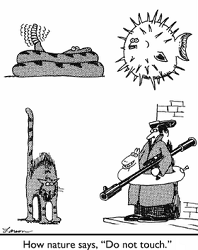
\includegraphics[width=\figwidth]{pics/19/26.png}
	\end{center}
\end{wrapfigure}
Twitch practically cried when he cracked open the first crates (plural) of detpacks, mines, razorwire, grenades, other types of grenades, and assorted anti-armor ordinance. 
The rest of us were a bit more interested in the box containing half a dozen excellent-quality Hotshot Lasguns (with full attachments) and a nice standard, Guard-issue, hopefully machine-spirit-free, Plasma Gun. 
Tink's modified Astartes weapon was gleefully tossed into the nearest trashcan, which immediately caught fire. 
He was less happy when Sarge made him put out the trash fire, fish the gun back out, and then strip his modifications and get the thing re-consecrated. 
Y'know, just in case any Space Marines came asking for it for later. 
There was probably a limit to how much Astartes wargear we could "misplace" after all.

Anyway, once Twitch was resupplied, the ensuing frenzy of fortification was everything we'd wanted over the weeks in that damn hab. 
It did wonders for our relations with the Military Police too: 
just one little incident was all it took for them to decide they'd rather submit politely worded notes via post instead of banging on our door in the middle of the night. 
Of course, there were some raised eyebrows up in the local brass, but a little extra fortification is far from the oddest thing a visiting guard regiment has done (especially if you include feral-world regiments or Ogryns), so they didn't kick up too much fuss and Sarge got them sorted in exchange for a promise not to extend the perimeter any farther. 
As for the one particularly annoying PDF Commissar who started poking his nose where it wasn't welcome (possibly for the same Nubby-related reasons the MPs had been), a short chat with Twitch and our "Valhallan Auxiliary" convinced him he really didn't want any part of our craziness. 
In fact, he seemed firmly convinced we should be kept as far away from his troops as possible, just in case we were contagious or something.

\begin{wrapfigure}{O}{\figwidth}
	\begin{center}
		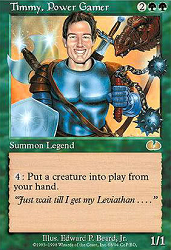
\includegraphics[width=\figwidth]{pics/19/27.png}
	\end{center}
\end{wrapfigure}
Aside from a bit of cogitator work for Sarge, Tink primary job was gear prep, which included a little pet project he'd been planning for years now. 
See, despite not being nearly as paranoid as Twitch, our techie still embraced the old Guard motto "Have a plan to kill everyone you meet, preferably from as far away as possible". 
Ever since his first mission under Bane and its anticlimactically blood-free ending, he'd been idly chewing at the problem of how to deal with someone capable that level of bullshittery. 
Skipping over some of the more harebrained stuff, one of his more promising ideas was a way to counter all the misfires, jams, and plasma-related mishaps that plagued anyone firing a weapon in Bane's weird probability-skewing "danger zone". 
His solution had something to do with choosing, tuning, and using weapons in a way the provided maximum damage for minimum danger, or "Max/Min-ing the Danger Per Shot" as he put it. 
Honestly, none of the rest of us really followed the fine details, or understood why Tink needed so much firing range time, or so many boxes of assorted weapons (including the oldest, most used lasguns in the range's armory for some reason), but Doc assured us it was all very "scientific".

In addition to translating and mediating for Tink (especially when the techie's request for "a platoon of your slackjawed PDF yahoos to fire these guns for me" raised issues with a decidedly non-slackjawed Range Officer) Doc was put in charge of liasing with our Inquisitorial comrades. 
Well, more "spying on" than "liaising with", but anyone who's been an LSO can tell you it's practically the same thing. 


\begin{wrapfigure}{O}{\figwidth}
	\begin{center}
		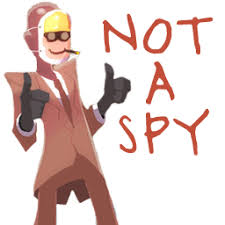
\includegraphics[width=\figwidth]{pics/19/28.png}
	\end{center}
\end{wrapfigure}
Scisistat wasn't returning our calls and our former team had relocated from the hab base without leaving a forwarding address. 
The other team hadn't moved though, and over the next two weeks Doc occasionally drove over to chat with their friendly old adept/surgeon about our former teammates' health and all the medications Ivana wasn't taking. 
For some reason his visits just happened to coincide with the times when everyone else was out of the base, and it always seemed that either the Fringe Worlder or Torso-priest had left a copy of their latest briefings lying around the medbay. 
The fact that Doc's half-assed espionage got us MORE intel that we'd ever gotten while on Sciscitat's actual bloody team should really illustrate the man's opinion of us.

In any case, most of the stuff Doc got was about the stupid artifacts, which were decidedly Not Our Problem, but there were some useful tidbits on The Sorceress too. 
Between what he got and Sarge's stuff on Bane, we had more than enough to get started with, and before long The Plan began to really take shape. 
The basic theory hadn't changed much since its initial inception, but since it was cooked up by a bunch of tired, shot-up grunts in the back of van, on their way home from a catastrophically failed op, that probably wasn't something to brag about. 
In any case, the first step was splitting our targets up. 
Bane was threatening enough on his own, we shuddered at the thought of what he could do if someone with an actual functioning brain was calling the shots. 
Of course, of the pair he'd be the easier one to distract (and Tink had a surprisingly good idea for that), the problem was that Angelica knew this too and was good about keeping an eye on him. 
We needed to fix that.

\begin{wrapfigure}{O}{\figwidth}
	\begin{center}
		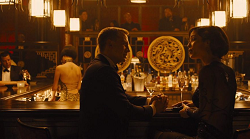
\includegraphics[width=\figwidth]{pics/19/29.png}
	\end{center}
\end{wrapfigure}
Now, it wasn't like little miss traitor-pants was always hanging on Bane's arm, in fact she left him to his own devices fairly frequently (which we felt disproved Ivana's assertion that she was "compromised" too). 
We weren't exactly sure what she was doing during these absences, probably plotting treason or enacting dark rituals (which Bane would find boring), or maybe she was off "negotiating" with various powerful male figures who'd respond poorly to her boy-toy's presence. 
In any case, whenever Angelica went off on her own, she always dropped Bane off at a certain up-hive club (which we dubbed his Daycare), along with at least one of her doubles and a few other helpers, who presumably were just there to call her whenever he got bored and wandered off. 
So far she'd always arrived on the scene and sidetracked him before he managed to overloaded a hive's fusion reactor or something, but it was probably only a matter of time.

The point is, that before we could neutralize Bane, we'd need to arrange for Angelica to be distracted too. 
The problem was that there were only a very limited number of things that would get her attention, five of them to be specific if Scisitat's little briefing on his stupid artifacts was to be believed...

This might've been the point where we started to go a just little off the rails. 
Well, at least according to our defense counsel.

\begin{wrapfigure}{O}{\figwidth}
	\begin{center}
		
\includegraphics[width=\figwidth]{pics/19/30.png}
	\end{center}
\end{wrapfigure}
I mean, it wasn't like we set out intending to steal the artifact. 
It was just that, of the the five, Angelica and Bane already had two (the Crime Lord's and another they'd gotten earlier), then there was the one we'd blown up (ON ORDERS), and finally one Ivana said her team had retrieved, which meant Sciscitat had it now. 
This just one left spooky artifact out in the wild, and we didn't much like our chances of getting to it before the people who were, you know, actually trained for that stuff.

We did look into other options, such as Twitch's perfectly reasonable idea of mining all routes out of the upper hive and just waiting until Angelica found the last artifact herself. 
The problem was that even though the number of routes between hives was limited by the massive rock-storm (it stops being sand or dust once it's bigger than a grape), there couldn't possibly mine ALL of them. 
Well, actually we probably could, we were beyond well stocked at this point, but you can't just leave massive piles of explosives lying around on pieces of crucial hive infrastructure... 
someone might steal them. 
Anyway, if she found an artifact on her own, she'd probably bring Bane with her, which was exactly what we were trying to avoid here.

We also toyed with the idea of just creating a fake artifact, which we could be sent some place Bane wasn't welcome, such as that Merchant Cartel. 
One of the reports Doc had gotten had a few pictures of the last artifact (another spooky box thing), and Tink was fairly certain he could rig up a close enough duplicate out of cardboard or something. 
Even better, since there wouldn't be any actual artifact stuff inside, we could just pack box itself full of explosives. 
Both Sarge and Doc vetoed this idea on the grounds that it involved the words "fairly", "close enough", and "cardboard". 
Also, she was a psyker and would presumably be able to tell the difference between an ancient eldritch artifact and a forgery, regardless of quality. 


\begin{wrapfigure}{O}{\figwidth}
	\begin{center}
		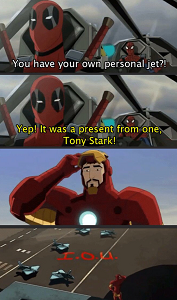
\includegraphics[width=\figwidth]{pics/19/31.png}
	\end{center}
\end{wrapfigure}
Ivana even put forward a whole nother option for bait: 
Inquisition agents, specifically us. 
After all, she reasoned, if Angelica hated us so much, she was sure to come down to personally tear our limbs from our bodies and crush our skulls with her bare... 
hands. 
At least, that's what Ivana would do. 
We (very, very cautiously) explained that while this was an excellent idea, and everyone appreciated her suggestion, A: 
we'd been bait before, and hadn't much liked it B: 
No, she wouldn't come anywhere for us. 
She might send Bane, or have an orbital strike called in, or send the entirety of the Secret Police, but we highly doubted she'd show up in person. 
Even to gloat. 
At least not until we were all good and dead. 
Now, if it was Sciscitat on the other hand, or maybe one of his favorite minions... 
well, that was something worth thinking about. 
Or it would've been, if we weren't TOTALLY ABOVE THAT SORT OF THING.

So we really did our due diligence on this, but we just that we HAD to get an Artifact of our own, and of the four still existing we only knew where one of them was. 
It was, inevitably, Nubby who raised the question of if, you know just hypothetically, Sciscitat REALLY needed his. 
After all, if Angelica and Bane were dead, wouldn't that practically solve his whole scavenger-hunt problem for him? 
It would be for the Greater Good, as the Tau weirdos would say.

\begin{wrapfigure}{O}{\figwidth}
	\begin{center}
		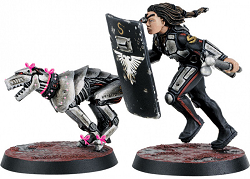
\includegraphics[width=\figwidth]{pics/19/32.png}
	\end{center}
\end{wrapfigure}
The saner members of the squad watched in increasing alarm as first Twitch, then Tink and Ivana chimed in to add their support, and began planning was quite possibly the most harebrained heist in Inquisitorial history. 
When they got to the part with the clown masks and the giant wooden badger, Sarge finally put his foot down. 
He stated, in no uncertain terms, their heist was the exact sort of stupidity we'd been fighting with since we'd been "volunteered" for Inquisitorial service, and that wasn't even touching on the fact that we didn't actually know if the artifact was still in the other team's base, or how shaky our plan for baiting out ONLY Angelica was; 
we were not even remotely qualified for this sort of thing. 


Fortunately, we knew a few people who WERE. 
Admittedly they were the exact same people we were planning on stealing the artifact from, but that just put them in a uniquely good position to get it for us. 
All we had to do was convince one or two Sciscitat's minions to sell him out, and according to Ivana, there was one specific person who was uniquely primed to do just that: 
his Interrogator. 
Sure, she seemed to be the man's most loyal follower, and probably hated our guts even more than he did, but if what Ivana said about her being "compromised" was true... 


At first we hadn't put much stake in Ivana's whole "compromised" thing, but then the other team's surgeon asked Doc for a consultation on the Ganger, who'd been kept in medical confinement ever since her encounter with Bane. 
It hadn't been pretty: 
the trash-talking, mohawk-sporting, gun-nut who'd reminded us so much of Aimy had been reduced to something like a strung-out Obscura junkie, except somehow so much worse. 
Every conversation with her inexorably turned to Him, had Doc seen Him, did Doc know anything about Him, had Doc MET Him? 
When Doc had come back, he had a quiet word with the rest of us about taking Ivana more seriously, which we did (not that he much liked the end result).

\begin{wrapfigure}{O}{\figwidth}
	\begin{center}
		
\includegraphics[width=\figwidth]{pics/19/33.png}
	\end{center}
\end{wrapfigure}
Mind you, even if Ivana was right and the Interrogator was just as brain damaged as the Ganger (only a lot better at hiding it), that didn't mean she would go steal us an artifact just because we asked nicely. 
We needed to phrase our request just right, make it clear that all we wanted the Artifact for was to kill Angelica, you know, the Evil Manipulative Sorceress controlling poor impressionable Bane Johns. 
We certainly didn't have any desire to try and kill HIM (we were a bunch of cowards after all). 
Hell, with someone more, um, Interrogator-like guiding him, he might just be willing to come back to Inquisitorial service! 
That would never happen if Scisitat got his way though, all he cared about was his Artifacts, once he got them he'd just run off again, leaving Bane under Angelica and the Conspiracy's control...

Yeah, the real problem was't so much the phrasing as keeping a straight face, especially since it would be Doc doing the delivery. 
Which is why, instead of making his pitch to the Interrogator directly, he went and visited the one person even more "compromised" than she supposedly was. 
Doc wasn't very happy with his role in Operation Exploit The Mentally Traumatized For Strategic Gain, but he grudgingly made one last trip to the other team's base. 
With the equally grudging help of their Surgeon, our medic had the most obviously staged conversation in the history of espionage in front of the Ganger, who briefly "escaped" during the Interrogator's next visit to their base. 
The fact that this all somehow WORKED was mind boggling.

A few after Doc's visit we received a calligraphed note informing us a "distraction" would be drawing the Sorceress' personal attention to Jack Hive. 
Day after tomorrow.

\begin{wrapfigure}{O}{\figwidth}
	\begin{center}
		
\includegraphics[width=\figwidth]{pics/19/34.png}
	\end{center}
\end{wrapfigure}
Two days of frantic scrambling later, Sarge and Ivana were in position on a maintenance walkway overlooking Interchange 7JU-4, trying to look as bored and PDF-like as possible, and hoping their heavy weapons weren't visible from the lanes below. 
Across the way, Doc was leaned against an inappropriately camo-netted lascannon, desperately trying to ignore Nubby's dissertation on the inherent deviousness of all women. 
Above both groups, perched on the network of pipes clinging to the underside of the junction's 16-lane northbound overpass, Twitch sat with his pile of detonators, watching the incoming traffic like an especially jumpy hawk, and periodically rechecking the distance markers he'd placed along the roadside. 
Thirty kilometers away (some of them vertical), Tink double-checked his comm connection to the "auxiliaries", watched his chrono tick down to 0, and stepped into Seven Hive's most famous club. 
He then sheepishly stepped back out, and proceeded around to the service entrance before the bouncer tore his head off.

At T plus fifteen minutes, Tink had changed into his disguise, delivered his package, and was in position in the discrete spot the bribed paparazzi had told him about. 
At twenty, one of the lookouts Nubby had hired ("onrably 'tired PDF vet'rans, evry one of 'em") reported a flier with a Planetary Government IFF transponder landing, and a man with a "real fancy lady" exiting. 
Tink switched his dataslate over the appropriate feed, and immediately recognized Bane and Angelica, and switched to visual as they entered the club proper and proceeded to their usual spot. 
He watched them careful as they settled in and ordered drinks, patiently waiting for the moment when Angelica would quietly slip away. 
Then he kept waiting.

\begin{wrapfigure}{O}{\figwidth}
	\begin{center}
		
\includegraphics[width=\figwidth]{pics/19/35.png}
	\end{center}
\end{wrapfigure}
Over an hour and three false alarms later, Sarge commed Tink to check what was taking so long. 
The techie in turn called his increasingly annoyed observers to check for the ninth time whether any vehicles with the appropriate "fast lane" tags had left the garages. 
He got a combination of drunken slurring, hacking coughs, mutters about shrimp, and quacking, which equated to a firm "no". 
Except from the landing pad team, who angrily (not to mention drunkenly) told him they hadn't seen anyone AT ALL since the flier that dropped Bane off, the one with the hot pilot, had left to park somewhere else. 
Tink briefly considered the merits of mass hobo murder, possibly followed by suicide, especially when his "observers" explained that no, they hadn't watched where it went, they'd been diligently keeping their IFF readers pointed at the pad and waiting for Tink's word that the target was leaving. 
After a few deep calming breaths, he called Sarge back to let him know there might be a problem. 
Sarge did not take it well.

In the face catastrophic mission failure and an enraged noncom's inexorable wrath, Tink did what came naturally: 
loudly complaining about how it wasn't his fault. 
He was the ONLY one of us who hadn't been on the whole Angelica mission, he'd only seen her the one time at the Crime Lord's place, how was he supposed to tell if it was her or a double? 
And anyway, it was NUBBY who hired a bunch of random drunken bums to be our spotters. 
None of it was Tink's fault, his part of the plan was actually working just fine, Bane had already gone through three bottles of the exceedingly fancy stimulant-infused liquor Tink'd delivered, and he was ready to put his distraction into play at a moment's notice. 
In fact he could do it right now, with or without the double there, because HIS plans ALWAYS worked. 
Sarge just screamed at him to do absolutely nothing without further orders, and then cut the comm. 


\begin{wrapfigure}{O}{\figwidth}
	\begin{center}
		
\includegraphics[width=\figwidth]{pics/19/36.png}
	\end{center}
\end{wrapfigure}
In the pained silence that followed, Doc quietly told Sarge it was probably time to call Scisitat and tell him what was happening. 
He could actually hear the noncom's teeth grinding from from the far side of the interchange, but didn't get a response. 
Rather than argue, the medic just sighed, dialed his long-range comm to the Surgeon's number himself, and asked her forward him up the line. 
He'd gotten as far as the Torso-priest (who's immediate response was to ask what we'd fucked up), before Sarge finally manned up and grudgingly took over the call.

Now, Sarge had been embarrassed before, in fact since joining the Inquisition he'd been "the most embarrassed he'd ever been in his entire life" on several occasions. 
It didn't seem possible, surely there was some upper limit where you'd actually literally die of it, but somehow he kept managing to reach new heights. 
His conversation with Sciscitat, admitting we'd lost the Sorceress, who was probably halfway to Jack Hive to pick up "an" Artifact, maybe just possibly from the Cartel's subspire, was one of those moments. 
(He did at least manage to remember the old Diplomacy Adept's advice about admitting things, but it was a bit of a moot point, since the Inquisitor's first words were "It was YOU!")

Actually, skipping over the abuse, mockery, and general Angry Inquisitor Noises, Sciscitat took it surprisingly well. 
He eventually confirmed Angelica's arrival in Jack Hive via the governmental vactrain and her acquisition of the Artifact, and agreed to track her for us. 
He even grudgingly admitted that we'd chosen the best spot for our ambush, which was vaguely worrying given we'd never told him that. 
He instructed us to hold position and refrain from contacting him again, he'd let us know when Angelica was on her way back, and would provide tracking information once she was in our hive, but in the meantime he had far, far more important things to do. 
Sarge accepted this as gracefully as he could manage.

\begin{wrapfigure}{O}{\figwidth}
	\begin{center}
		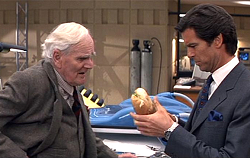
\includegraphics[width=\figwidth]{pics/19/37.png}
	\end{center}
\end{wrapfigure}
Despite Sciscitat's assurance he'd warn us in time, the wait was absolutely nerve-wracking. 
Tink had the worst of it, sitting across from an increasingly drunk Bane and the Angelica look-alike. 
He was on the verge of activating the distraction himself, whatever Sarge said, when the 30-minute warning finally came through. 
The techie breathed a sigh of relief as he finally got the word Go, re-donned his white coat and cheap wig, and did one last check to make sure he had the right address for the Arbite's Precinct Fortress.

Bane Johns, Interplanetary Man of Mystery, Lovable Rogue, and All Around Badass had been having an okay night all things considered. 
Sure, Inquisitor Girlfriend had ditched on their date, and the arm-candy was being especially fussy tonight, but the new drink they were serving was absolutely amazing. 
He was definitely getting bored though, and the chick was starting to really harsh his groove. 
Maybe it was time for a nice walk, he always found something interesting to do when he went for a walk. 
Inquisitor Girlfriend would nag him afterwards, but she never stayed mad, she understood a man as awesome as him had Needs. 


Bane was about to ditch when what's-her-name got all bothered about something and left on her own, he didn't worry about it, chicks did that sometimes when he was bored of them. 
He was on his way to the windows (doors were so passe) when a little old guy with a briefcase in one hand and a huge bottle of that new drink in the other walked up to him. 
He thought the guy looked a bit familiar, but he stopped worrying when the geezer pressed the bottle into his hand and opened up the case. 
Bane eyes lit up as he took in the impressive array of gadgets, beautiful pair of autoguns, and reconnaissance photos featuring a sinister-looking building and a nicely filled out young woman.

\greentext{>"The Planetary Governor's hot daughter has been kidnapped by ninjas. Are you a bad enough dude to save the Planetary Governor's hot daughter?"}


\begin{wrapfigure}{O}{\figwidth}
	\begin{center}
		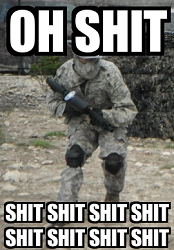
\includegraphics[width=\figwidth]{pics/19/38.png}
	\end{center}
\end{wrapfigure}
Sarge grinned with relief as his PDF-issue scanner picked up the first confused chatter on Arbites' bands. 
He reminded Tink to return as soon as he was sure Bane didn't need any more combead prodding, and turned his full attention to the ambush. 
According to Sciscitat, now that Angelica had her prize she was travelling in a six-vehicle semi-armored Secret Police convoy. 
Not that the armor would do much good against the literal crates of high explosives that'd been crammed under the interchange. 
Admittedly there was going to be a bit of collateral damage, but this was Inquisitorial business; 
the civvie body count would be positively miniscule compared to, say, an Exterminatus. 
The noncom was doing a final weapons check with Ivana (not that they'd really be needed once the explosives had done their bit), when he received the final awaited from Sciscitat.

What Sarge, and the rest of us, were expecting was a last minute update on which of the reserved lanes under us Angelica would be taking. 
What we GOT was a slightly-breathless warning from the Inquisitor that the convoy had started turning towards Underhive, possibly to take the Artifact to some secret warehouse instead of the Secret Police HQ, Bane's nightclub, or even the Arbite Precinct, like we'd planned for. 
She'd still be passing through the interchange, just on a completely different, and far lower, section than the one we'd set our ambush on... 
Sarge didn't even stop to swear, there wasn't time and he didn't know any words vile enough for the current SNAFU anyway, he just grabbed as many Krak launchers as he could carry and started sprinting along the walkway. 
Ivana shrugged and jogged after him, carrying their heavy bolter one handed and humming to herself.

\begin{wrapfigure}{O}{\figwidth}
	\begin{center}
		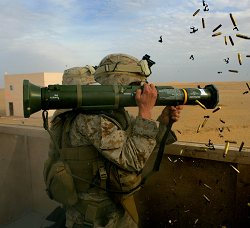
\includegraphics[width=\figwidth]{pics/19/39.png}
	\end{center}
\end{wrapfigure}
On the far side of the interchange from Sarge and Ivana, Doc hastily plotted a slightly longer route down to the new ambush point, and dragged Nubby away from the lascannon before the trooper could voice any complaints about how much it'd cost. 
Twitch watched them go from his perch above the interchange, spent a few seconds debating whether it'd be worth setting off his charges anyway (just in case some stray debris knocked out the lower section), and regretfully ditched his neatly arranged rows of detonators. 
As the demolitions trooper attached his rappel gear, he warned the rest of us that he was going to be a little late to the party. 
Doc suggested he meet up with Tink, who was racing back towards us on a PDF messenger bike, simultaneously trying to dodge slower traffic, direct Bane to the Arbite Marshal's office, and take off his Quartermaster Agent disguise. 
Tink tried to reply, but it just came out as inarticulate cursing.

Sarge skidded into position just in time to see the convoy's lead vehicle round the corner, he signaled Ivana to keep moving and get a better firing position while he started prepping his three Kraks for rapid fire. 
A distant corner of his mind registered a voice on his combead instructing him to call off the ambush so Angelica could be tracked to her Artifact warehouse, he instructed the voice to go have relations with several varieties of farm animals, sighted his first Krak on the middle of the section, and started counting down. 
Farther along the walkway, Ivana found a security door marked "stairwell" and casually kicked it off his hinges. 
One of the startled maintenance workers inside informed her that she couldn't do that, realized he was very obviously wrong about that and stepped aside, his partner didn't and regretted that decision for the rest of his life. 
Ivana reached the level above the roadway a few seconds after the maintenance worker, but unlike him, she stopped there and exited right as Sarge's countdown hit zero.

\begin{wrapfigure}{O}{\figwidth}
	\begin{center}
		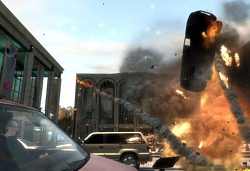
\includegraphics[width=\figwidth]{pics/19/40.png}
	\end{center}
\end{wrapfigure}
The first Krak missile was right on target, it punched through the "armored" glass of the lead car's windshield like wet paper, reducing the vehicle and its occupants to flaming wreckage before they even registered the attack. 
The second car, driving slightly farther back and left in the other reserved governmental lane, spun out as it tried to evade and cartwheeled a good fifty meters before it came to a stop. 
None of its occupants got out before Sarge's second Krak hit its exposed undercarriage.

The rest of the cars in the convoy, including the more-heavily armored limo in its center, reacted professionally enough, but they were in a remarkably shit tactical situation. 
There were obvious advantages to taking the governmental fast lanes, with their secured entry points and the chest-high barrier separating them from the common rabble clogging the rest of the highway, but the disadvantage was being pretty much trapped in a two lane killbox. 
The only smart move available was to try and bust through the wreck of the first cars and keep moving, but three more Kraks (Sarge's last one, and two from where Doc and Nubby had just come out on the wall above them), were enough to completely block the way. 
With a massive pileup of other governmental vehicles already blocking way behind, the Secret Police took the only option left to them, and started getting out to return fire.

\begin{wrapfigure}{O}{\figwidth}
	\begin{center}
		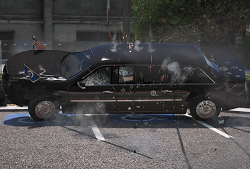
\includegraphics[width=\figwidth]{pics/19/41.png}
	\end{center}
\end{wrapfigure}
From her slightly elevated position and across the highway from the convoy, Ivana opened up on the disembarking Secret Police with her heavy bolter, greatly increasingly the panic level in the eight lanes between them. 
Above her, Sarge cursed himself for not bringing any more Kraks or his nade launcher, and started trading las-fire with the well-covered men below. 
He didn't land many hits, but between him and Ivana they had the entire convoy nice and distracted for Doc and Nubby's follow-up attack.

After a short debate over targets, Doc and Nubby decided it'd be best to stick to the objective, and two Krak missiles slammed directly into the roof of the still-unopened limo in the middle of the convoy. 
Admittedly it was a bit overkill given they were firing anti-tank ordinance, but the two guardsmen felt it was best to play things safe. 
You can imagine how surprised and disappointed they were when the smoke cleared to reveal a burned, battered, but still intact limo, now glowing with a faint pinkish-purple light. 
Lacking any better ideas, Doc and Nubby started tossing grenades as fast as they could grab them, hoping for a lucky hit with a Krak nade or something, but only managed a few glancing hits before return fire from the Secret Police fire forced them back into cover.

It was at this point that the fight began to stall. 
As well as our opener had gone, we'd blown all our hole cards. 
There were still at least ten Secret Police agents still standing and their armored cars made damn good cover, even from grenades. 
We had them pinned, but time was on their side and they knew it, we only had so long before reinforcements started pouring in and we'd be in all sorts of shit. 
Nubby suggested a run back for more Kraks, and Doc wanted to wait for Twitch and Tink, but Sarge vetoed and gave the order to advance. 
It really said something about the situation that nobody objected.

\begin{wrapfigure}{O}{\figwidth}
	\begin{center}
		
\includegraphics[width=\figwidth]{pics/19/42.png}
	\end{center}
\end{wrapfigure}
As Sarge dropped down and began pushing through eight lanes of semi-stalled traffic, and Nubby and Doc left their nice safe drainage pipe to take turns sprinting down the exterior stairs below them, Tink finally reached the interchange. 
The techie cut off his call to Bane with a final hammed-up death-gurgle and directions to "avenge him" and tried to figure out just where the hell in the giant concrete rat's nest the fight was. 


Tink's attempts to get directions from his distracted teammates were interrupted by someone dialing his combead directly and screaming "STOP THIS TRUCK" in his ear. 
Tink looked around in confusion, eliciting more more yelling, before he finally spotted a tanker wallowing through traffic next to him with a small figure jumping up and down on top of it. 
Tink took in the size of the tank, the bright red FLAMMABLE markings on its side, and the detpacks in Twitch's hands. 
The techie then briefly tried to remember how many crates of explosives they'd packed in the bridge he was currently riding on, before giving up and weaving through traffic towards the tanker with a shout of: 
"Ohhhh shit Twitch, you're gonna get us all killed."

The surviving agents of Task Force Spectre, handpicked by the Inquisitor herself to act as her last line of defense, let out a ragged cheer as the mystery attackers suddenly began pulling back. 
Their cheers were cut short by a massive crunching sound above them, and they looked up nearly eight levels to the overpass above them and the truck cab hanging over its edge. 
All nine agents watched, too stunned to even notice a chunk of debris that flattening their commander, as the truck teetered on the lip for a second, before finally tipping and dropping directly towards them. 
The limo's occupant, unsure what was happening, peaked out the door for a second, before slamming it shut and pouring every ounce of her newfound powers into her shield.

The tanker was about ten meters off the ground when the detpacks on its side detonated it in a massive, oddly wet-sounding FWOOP.

\begin{wrapfigure}{O}{\figwidth}
	\begin{center}
		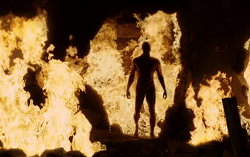
\includegraphics[width=\figwidth]{pics/19/43.png}
	\end{center}
\end{wrapfigure}
The explosion was big, just not as big as we'd expected, which was honestly a good thing given how close to it some of us were. 
Instead of the massive fireball and concussive shock we'd expected, what we got a flaming spray like the world's largest incendiary grenade, covering the entire highway in burning... 
fuel. 
The smell was, well, familiar.

Up on the overpass, Tink turned to the man next to him, who was looking over the edge with the rapt expression of someone who'd always wanted to that. 
He read, then re-read the word's "No Shit Services: 
For All Your Septic Needs" on the man's coveralls, then looked at Twitch, who shrugged and muttered about it being the best he could find; 
Tink shook his head. 
Both guardsmen hooked their drop harnesses to the railing and rappelled down into the quite literal flaming shit-show below. 
The septic worker saluted them.

Sarge was the first to arrive at the smoking epicenter of the explosion, but the rest of us weren't far behind. 
As we arrived we heard a faint melodious voice cursing and screaming somewhere inside the flames and smoke, then a blast of lightning knocked Sarge off his feet. 
The singed noncom spared a second to thank the Emperor for carapace armor, and rolled into cover while the rest of us sprayed fire into the smoke, somewhere inside Angelica screamed something eldritch sounding and daemonic figures started rising out of the muck. 
At least we thought they were daemonic, it was hard to say, because we just kept shooting, taking them out before they could finish forming. 
I mean, we'd seen this trick what? 
Fifty times now? 
A hundred? 
Angelica and her bullshit might've been intimidating back in the early days, but after spending a few months with the Daemonthrope, well... 


\begin{wrapfigure}{O}{\figwidth}
	\begin{center}
		
\includegraphics[width=\figwidth]{pics/19/44.png}
	\end{center}
\end{wrapfigure}
As we mowed down the whatevers-they-weres (NOT shit-daemons, whatever Tink said), Twitch and Sarge began tossing short-fuse frags into the cloud until we were finally rewarded with a pained yelp and a filth-splattered figure zipped out of the smoke. 
Once again Sarge was hit in the chest, except this time by two amazingly-aimed bolt-pistol rounds, knocking the burly noncom back a good two meters, and pretty much destroying what was left of his chest armor. 
He was still capable of swearing though, so Doc declared him stable, and joined the rest of us firing at the sprinting figure.

Angelica was moving at a fair clip, but her shield seemed to be failing and between three lasguns, a plasma gun, and Ivana's bolter we managed to tag her at least twice. 
She still managed to reach the maintenance door she was aiming for though, slicing through it with that sword of hers and rolling through the gap into the tunnel beyond. 
We followed at a more leisurely pace and felt a nice warm tingly sensation as she discovered it was a supply closet. 
It was quite possibly the most beautiful cursing we'd ever heard, in multiple ways. 


As all of us (except for Sarge who was still trying to remember how his legs worked) fanned out around the door, Angelica stopped cursing. 
In an impressively haughty voice given the circumstances, she announced that she had the Liber Demonica with her, and we'd never be able to kill her without destroying it. 
She informed us it was a stalemate, and instructed us to go get our Inquisitor so she could make a deal with im. 
Doc shrugged, looked over his shoulder and asked Sarge if he cared about any Liber Whatsits. 
The Acting Inquisitor told him where he could shove any stupid artifacts, and Doc passed that information on. 
Along with an entire bouquet of incendiary grenades courtesy of Twitch.

\begin{wrapfigure}{O}{\figwidth}
	\begin{center}
		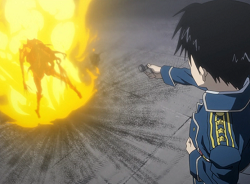
\includegraphics[width=\figwidth]{pics/19/45.png}
	\end{center}
\end{wrapfigure}
What came back out of the maintenance closet might've been ex-Interrogator Angelica Dominicus, but it sure as shit weren't human. 
Despite the claws, the tentacles in uncomfortable places, and all the flames, it was still somehow feminine though, and it moved with a familiar lithe grace. 
The voice though, that was something entirely alien, like a cross between honey and broken glass, accompanied by an invasive pulsing *something*. 
We stared in shock, as whatever it was pressed inwards trying to worm its way in through our ears, but only for second. 
Before it'd taken its second step, all six of us, including a slightly unsteady Sarge, opened fire. 
It got three more steps, but not four.

We only stopped firing when we ran dry, by that point there wasn't much left but a smoldering pulsating lump. 
While the rest of us reloaded Nubby, in violation of seventeen varieties of common sense, took a few steps forward to inspect the pile. 
He stopped short as a familiar pained voice called his name, and asked him to save her. 
The trooper looked down into the somehow-intact face and eyes of ex-Interrogator Angelica, who smiled at him and called him her knight in shining armor. 
Nubby smiled back, and informed her "it wasn't working out". 
Twitch offered her another incendiary boquet as consolation.

\begin{wrapfigure}{O}{\figwidth}
	\begin{center}
		
\includegraphics[width=\figwidth]{pics/19/46.png}
	\end{center}
\end{wrapfigure}
As much as we'd have loved to sit and watch our ex-boss' remains smolder in the hive-light, there wasn't time. 
The ambush had only taken a short while (only about a dozen or two "rounds" as us professionals call them), but the Secret Police had to have reinforcements on the way, and they probably wouldn't call things off just because their boss was dead. 
Even more worryingly, the combead Tink had given Bane was completely dead, and we could overhear chatter about SOMETHING leaving the Arbite's HQ at high speed.

It was time to get moving and, if possible, avoid dealing with any freakishly powerful secret agent types until we'd at least had time to patch ourselves up. 
Sarge, with a bit of support from Ivana, led the way back towards their side of the Interchange, where the faithful cargo truck had been stored. 
As we moved the noncom put in a courtesy call to Sciscitat to let him know Angelica was dead, but didn't get through, so he had Doc leave it with the Surgeon instead (no mention was made of any spooky Liber things though). 
We were just entering the stairwell when a high pitched whining sound drew our attention up towards the top of the interchange.

An Arbite Eagle shuttle, pouring smoke from its engines and weaving a tad drunkenly, shot down out of the sky, caromed off two walls, a support pillar, and a truck full of mattresses and a physically improbably manner, and skidded to a halt in the general vicinity of the maintenance closet. 
From the far side of the traffic, we heard a distance, surprisingly heartfelt-sounding

\greentext{>NOOOOOOOOOOOOOOOOOOOOOOOOOOOO}

\greentext{>*breath*}

\greentext{>OOOOOOOOOOOOOOOOOOOOOOOOOOOOO}


As the pitch rose and got angrier, Sarge instructed the rest of us to move faster.

\begin{wrapfigure}{O}{\figwidth}
	\begin{center}
		
\includegraphics[width=\figwidth]{pics/19/47.png}
	\end{center}
\end{wrapfigure}
So no shit, there we were, standing just across the street from a grief-stricken psychically-superpowered (self-proclaimed) secret agent. 
A man who'd killed at least two Inquisitors, single-handedly blown up an entire warp-ship, tackled an Ork Freeboota with nothing more than a pocket-knife, and had just spent the last hour shooting up the planet's Arbite HQ FOR FUN. 
A man who may or may not have been a daemonhost, and was shacked up with quite possibly the most dangerous woman we'd ever met, until she'd been killed. 
By us. 
Very, very thoroughly.

We decided it was time to start running.

The plan was still to kill Bane of course, it was just that we didn't particularly feel like doing it RIGHT NOW. 
We felt like we deserved a few hours off to grab a bite, get some light medical treatment, and maybe catch a quick nap; 
the universe felt otherwise. 
As we piled our way into the stairwell Bane's dramatic moment was cut short by the arrival of a squad of Arbite float-bikes (two of which spontaneously collided mid-air), and a very one-sided gunfight started moving straight towards us. 


Still though, we could think of a dozen places we'd rather duke it out with Bane than the middle of a packed highway covered with burning sewage (and directly underneath a MASSIVE pile of explosives), so we started sprinting up the stairs anyway. 
We pushed our way past a few confused emergency services types, including a pair hauling a broken-legged maintenance worker, up to the level that led to the garage where we'd parked. 
At this point Tink did some quick math, called a halt, and informed the rest of us that it was time to ditch our more unreliable assets before they became a liability.

A dozen levels below us, Bane Johns kicked the last of the Arbites through the maintenance door, and entered the stairwell at about the same time as 37 assorted grenades reached his level.

\begin{wrapfigure}{O}{\figwidth}
	\begin{center}
		
\includegraphics[width=\figwidth]{pics/19/48.png}
	\end{center}
\end{wrapfigure}
The vast majority of the grenades either overshot, undershot, failed to detonate, or somehow bounced out the door past Bane, but judging by the swearing and faint "mawp"-ing sounds, at least one of the flashes must've hit the target. 
Not that being blinded stopped the man from opening fire, and somehow managing to hit the back of Doc's helmet, a tank of fire suppressant on one of the first responders' backs, and the crippled maintenance guy. 
Twice. 
Twitch hastily moved his explosives-filled pack around to his front side, and led the retreat down the foam-filled hallway (until Nubby passed him).

Nubby found the exit into the parking garage blocked by even more emergency service guys and a fire-truck. 
Time being of the essence, rather than ask nicely, the little trooper bellowed at them to make a hole, kicked two in the shins, and left the rest to Ivana and Sarge, who scattered the stragglers like bowling pins. 
As he passed, Twitch tossed his pack to a particularly nervous looking fireman and instructed him to "RUN, FOR THE LOVE OF THE EMPEROR, START RUNNING!" The guy took one look in the bag, started screaming, and did.

Our trusty cargo truck wasn't parked far away. 
Most of us piled in and started swapping gear and doing field repairs, both on our kit and ourselves, as fast as possible. 
Tink, looking around and taking in the number of explodable vehicles filling the garage, decided that this was just about the second worst place to fight Bane, and got in the driver's seat instead. 
Those of us in the rear were abruptly thrown to the floor, then the wall, and then the other wall, as Tink attempted to "drift" the six-wheeler down the garage's exit ramps before Bane finished whatever the hell he was doing to those poor fire guys. 


\begin{wrapfigure}{O}{\figwidth}
	\begin{center}
		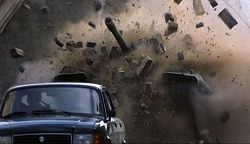
\includegraphics[width=\figwidth]{pics/19/49.png}
	\end{center}
\end{wrapfigure}
As we hit street, shedding the last of our explosives (and very nearly Doc) behind us, Tink took a second to congratulate himself on his genius and floored it. 
He then yelped and attempted to floor it even harder as a burst of static arced along his hands, the radio spontaneously played a 7-note sting, and the frickin firetruck burst through the parking garage's walls four levels above us. 
Bane, hanging out the door and driving one handed, grinned madly at us as he opened fire.

Fortunately his aim was a bit off: 
instead of pancaking us, the firetruck came down in the opposite lane, smashing directly into an oncoming truck and setting both off in a disproportionately large, purple-tinged fireball. 
His bullets were a bit wide of the mark too, or at least that's what we thought until two of our tires exploded. 
Tink swore and tried to maintain control, but only managed to hold for a few seconds before Bane, having somehow been propelled OVER us by the blast, took out both our front tires as well. 
There were a confusing and bumpy few seconds for those of us in the back as the Techie narrowly managed to avoid sending us over a looming drop all the way to underhive, somehow skewed us between a pair of oncoming busses, and finally plowed our sturdy vehicle through the side of one the buildings lining the road. 


Having unanimously decided it was time to get off Mr. 
Tink's wild ride, we disembarked and found ourselves in some sort of warehouse. 
Twitch hastily inspected the markings on the nearest crates for any warning stickers, didn't notice anything more sinister than "Munitorum-Grade Taco Substitute, Substitute", and declared the warehouse as non-hazardous as we'd get. 
Sarge gave the order to take up defensive positions.

Two minutes of tense waiting later, Tink made a "get on with it" gesture at Sarge, who just glared back. 
Ivana sighed, rolled her eyes, and announced that "Not Even Bane Johns Could Stop Us Now". 
The skylight above her exploded inwards.

\begin{wrapfigure}{O}{\figwidth}
	\begin{center}
		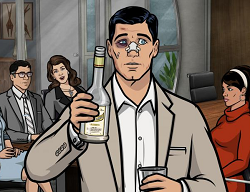
\includegraphics[width=\figwidth]{pics/19/50.png}
	\end{center}
\end{wrapfigure}
As Bane landed, we noticed the bastard wasn't quite looking his usual unruffled self. 
Back when we first came up with the whole distraction plan there'd been a bit of debate over who to sic Bane on. 
We wound up deciding that, given how much trouble a certain member of theirs had given us, the Arbites owed us a favor, and man did the boys in black deliver. 
While the bastard was still upright and looked suavely self-confident as ever, he'd collected a dozen minor scrapes and bruises, and from the look of things some (probably deceased) hero of an Arbite had popped him square in the eye with a shock-maul. 
Even more importantly though, the man was breathing heavily, and as he'd dropped down into the warehouse (without a rope or grav-chute) a distinctly warpy breeze had come with him. 
Just this once, we took that as a good sign.

Upon landing right in front of Sarge and Ivana, Bane launched into this whole spiel about how he didn't know who we were, or what we wanted, but he had a very particular set of skills, and so on... 
We all just stood there, listening to him monologue like a bunch of idiots, until Twitch abruptly snapped out of it and opened fire. 
The rest of us immediately shook whatever it was off and followed suit, pouring five lasguns' and one bolter's worth of fire after the man as dodged backwards behind a row of crates. 
None of the shots hit, of course, but we hadn't really expected them to, at least not yet. 
That killing part would come later, for now it was all about keeping up the pressure, which is why Sarge and Ivana pushed forwards after him, while the rest of us moved around the flanks to cut him off.

\begin{wrapfigure}{O}{\figwidth}
	\begin{center}
		\includegraphics[width=\figwidth]{pics/19/51.png}
	\end{center}
\end{wrapfigure}
The theory was simple: 
wear the bastard out. 
If this stupid "Danger Zone" of his really worked by skewing probability (or "stealing our numbers", as Twitch put it), then we were betting it took a lot more psychic juice to flip a 90-10 than a 50-50. 
Our goal was to put as much fire on him, as accurately as possible, and do it without leaving any handy options for his bullshit powers to work on. 
That last bit was where Tink's little secret weapon project came in.

At the end of his extensive testing Tink had handed each of us what had to be the oldest, wellest-used lasguns any of us had ever seen. 
They were completely unmodified, none of them matched, and we had no idea what pattern any of them were. 
We strongly suspected that they were all older than the Hive we were standing on, maybe even pre-Heresy, but it was hard to be sure since the serial numbers had been worn away ages ago (except for Sarge's, which still faintly read "-rge of Mars, SN: 
000-000-000-000-007"). 
Still, despite all appearances, Tink assured us they were the most reliable weapons on the planet, with only a single minor misfire between them in over two weeks of relentless test-firing. 
Twitch had immediately claimed the one that HAD misfired, asserting that the rest of ours were just ticking time-bombs, while Ivana had firmly refused to part with her customized Godwyn-De'az Bolter, claiming she'd had it for longer than she remembered. 
Tink wisely decided not to press her.

Of course, these "new" weapons didn't pack the same punch as our hotshots (or the shiny new plasma gun Tink had fired all of eight times before unceremoniously tossing out the truck's window), but the point was: 
when you pulled the trigger, a laser ALWAYS came out. 
Combine that with a lack of ricochets for Bane to pull his bullshit with, and it was all we could really ask for. 
Well, not really, but it was certainly all we were gonna GET.

\begin{wrapfigure}{O}{\figwidth}
	\begin{center}
		\includegraphics[width=\figwidth]{pics/19/52.png}
	\end{center}
\end{wrapfigure}
Rather than let Sarge and Ivana bum-rush him, Bane came around Doc and Nubby's side of the of the crates in a dive. 
The man was firing both his fancy little auto-pistols (not the specially inaccurate ones Tink had given him) on full auto, and somehow managed to simultaneously knock out a control line on one of Nubby's augmetic legs and hit Doc in both the shoulder and helmet, all before even hitting the ground. 
The pair's return fire missed wildly as Nubby's leg spazzed out and sent him plowing into the medic. 
Tink and Twitch, firing down the row, did considerably better though, forcing Bane into another acrobatic dive, this time "enhanced" by blast of howling wind which sent Doc and Nubby the rest of the way to the ground as he launched over them. 
Rounding the corner, Sarge and Ivana both took potshots at the magical flying Interrogator, and then sprinted after him as he passed behind a stack of boxes.

Sarge was still sprinting when he reached Bane's row, which turned out to be a mistake. 
The noncom threw himself into a dive, but misjudged his aim and plowed straight into a large shelving unit, catching four autopistol bullets and a small (but surprisingly heavy), crate to the groin in the bargain. 
Behind him, Ivana rounded the corner a bit more carefully, and stitched a line of bolt-rounds after Bane as he ran UP the same shelving stack. 
As admittedly cool as this maneuver was, it also took the man up into Tink and Twitch's line of fire, and the universe went slightly runny around the edges as the pair lined up their shots. 
For a brief second the warehouse was replaced by a screaming SOMETHING, with Bane hovering in the middle of it cackling, then Tink's weapon misfired. 
Twitch's didn't, and Bane dropped back down off the shelves with a girly little yelp as a lasbolt grazed his the thigh.

\begin{wrapfigure}{O}{\figwidth}
	\begin{center}
		\includegraphics[width=\figwidth]{pics/19/53.png}
	\end{center}
\end{wrapfigure}
Bane didn't hit the ground, not because he'd started flying again, but because Ivana caught him by the front of the tux and pinned him upside-down against the wall. 
The big woman grinned ear to ear as she shoved her bolter into his chest and pulled the trigger, only to pause and stare down in confusion as nothing happened. 
Even half-blinded with pain, Sarge could see what was coming next, and tried to shout a warning as, apparently forgetting years of guard training, she pulled the trigger again. 
The blast as first one bolt round, then the other, and then the entire rest of the magazine went off blew Ivana backwards through the opposite wall of crates, while somehow leaving Bane standing upright, wiping burning specks of propellant off his lapels. 


We didn't leave the smug bastard time gloat. 
Sarge rolled the rest the way to his feet and opened fire, only to swear as the warehouse was filled with daemonic whispers and HIS weapon jammed too. 
Operating on an only slightly better instinct than Ivana had been, the noncom hucked his ancient, supposedly unjamable, jammed weapon at Bane's face. 
He missed, of course, and Doc came around the corner just in time to catch four kilos of rapidly spinning metal to the nose. 
Fortunately, it didn't go off, and Bane was too busy laughing to even register Sarge's fist before it hit him in the gut.

Nubby, lagging considerably behind Doc, paused at the spot where Ivana had come to a rest, and since the medic was busy, promoted himself to Doctor Nubbs. 
He decided that, in his professional opinion, the patient needed thirty something-somethings of Slaught cut with Stimm, and maybe just a little Frenzon. 
You know, to take the edge off.

\begin{wrapfigure}{O}{\figwidth}
	\begin{center}
		\includegraphics[width=\figwidth]{pics/19/54.png}
	\end{center}
\end{wrapfigure}
Twitch and Tink entered the row to find Sarge in the middle of what might be described as a Kung-Fu battle. 
One that Sarge, despite being stronger, faster, and undoubtedly meaner, was definitely losing. 
Tink, confident in his ability to fire into melee, announced it was time to even the odds, and shot Sarge in the arm. 
Twitch suggested he not try that again and started moving closer.

Sarge, who was starting to really feel the broken ribs and blood loss, and was getting really tired of the little voice that kept promising him untold power in exchange for a small price, decided that enough was enough. 
As the bastard wound up for another of his stupidly effective chop-things, the noncom rushed into the blow and pulled his combat knife. 
He was very surprised when halfway through his attack everything went wobbly and suddenly the knife wasn't in his hand anymore. 
Sarge paused, perplexed, and tried to figure out where it had gone. 
It wasn't in his right hand, where it was supposed to be, and his left hand appeared to be missing entirely, which seemed a vaguely worrying. 
He directed his gaze downward, and was relieved to find the missing blade was merely lodged in his chest, he hadn't lost it after all. 
Secure in the knowledge that the Commissar wouldn't be angry at him for misplacing his wargear, the noncom decided it was time to sit down and take a quick nap. 
As he nodded off, he vaguely wondered if all the blood around him was his, and if he would be yelled at for making a mess.

On both sides of the row, Doc, Twitch, and Tink watched as Sarge staggered backwards and collapsed, and a rain of blood started falling from the warehouse's roof. 
All three of them looked up into the storm, then back down to where Bane was standing over Sarge, and opened fire.

\begin{wrapfigure}{O}{\figwidth}
	\begin{center}
		\includegraphics[width=\figwidth]{pics/19/55.png}
	\end{center}
\end{wrapfigure}
Things got very warpy, very fast. 
Whether it was the blood rain, and it's notorious effect on psykers, or just that Bane was finally running on empty, the man's powers seemed to go completely haywire as our barrage hit him. 
It started with a hive-quake knocking boxes off the stacks around us, followed by a psychic blast launching Bane into the air like a cannon, and then the nagging little whispers at the edge of consciousness abruptly growing into a full on assault. 
Tink dropped the ground, clutching at his head, but Doc and Twitch kept firing as Bane floated back down and bolts of warp energy started to arc around him, narrowly missing Sarge's prone form. 


Inside all the lightning, we could faintly hear Bane somehow simultaneously screaming, laughing, and arguing with someone about "how things work". 
Around him, tears in reality started forming, with indistinct hands and tentacles clawing at their edges. 
Twitch cursed his lack of explosives, tossed a vial of holy water at Bane (who didn't appear to notice), and yelled at the rest of us to keep shooting. 
Not that we needed telling. 
All of us, including a now-upright Tink and Nubby, poured as much fire as we could into the increasingly eldritch figure, and despite the age and piddliness of our weapons, it had a noticeable effect. 
Chunks of the man started burning off, whether from us or his own powers we couldn't say, but whatever he was turning into didn't seem to be able to regenerate. 
Yet.

As we kept firing and hoping for the best, there was a shout from behind Doc Ivana ran up gripping Sarge's lasgun. 
None of were quite sure what she was trying to do as she began advancing while hip firing (she was already in effective range), but whatever it was it sure as shit backfired. 
As she reached the ragged skeletal figure that was all that as left of Bane, the man's schizophrenic shouting was replaced by *something*, and a blast of bluish energy launched the woman across the room to land in a sizzling heap.

\begin{wrapfigure}{O}{\figwidth}
	\begin{center}
		\includegraphics[width=\figwidth]{pics/19/56.png}
	\end{center}
\end{wrapfigure}
When the flash of light faded, we found ourselves looking at pretty much the same thing, and not a four-story axe-wielding daemon, thank the Emperor. 
We were pretty sure the blueish veins covering what was left of his body were new though, same with the steadily growing horns and the feathery black wings. 
We responded to the sudden appearance of an actual, by all things unholy, DAEMONHOST, with the calm professionalism of true Inquisition agents and kept firing. 
Because honestly, what the hell else were we supposed it do? 
Run? 
FROM THAT? 
We knew a "die tired" situation when we saw one. 
And anyway even with his little upgrade Bane still wasn't looking that healthy, for all we knew it'd only be a few more shots before he keeled over. 
Right?

Well, actually the thing's next move certainly seemed in line with our assessment: 
instead of descending on us in a storm of daemonic fury, it waved a hand in the air and the warp rifts around us suddenly solidified. 
A creature that looked like a horrible amalgamation of twenty different creatures clawed out of the one nearest Tink and Twitch, while Bane himself started floating upwards to the largest rift the warehouse. 
Twitch and Tink immediately shifted their fire and began falling back, while Nubby and Doc kept dutifully kept on Bane, right until the arrival of a second interdimensional horror from a portal on their side of the row.

The hard decision of where to focus our fire, and whether to desperately try and kill Bane before we were clawed to death by his minions was a tricky one, especially without Sarge there to make it. 
Fortunately, before we dithered ourselves to death, the problem was simplified for us. 
Ivana, stained head to toe in blood (whether her's or the warpy stuff we couldn't tell) came screaming out from back of the warehouse and hit the slowly rising figure with a flying tackle, yanking Bane down away from the growing portal. 


\begin{wrapfigure}{O}{\figwidth}
	\begin{center}
		\includegraphics[width=\figwidth]{pics/19/57.png}
	\end{center}
\end{wrapfigure}
As we shifted our fire down to focus on our respective ravenous tentacular things, the blood-covered woman above us wrapped her legs around Bane's waist, grabbed one of his freshly-grown wings, and just tore it off. 
This got the thing's attention, to say the least; 
it responded by howling and clawing at her face and sides with sets steadily growing talons. 
She just ignored this and grabbed the other wing. 
The sound as it came off was... 
memorable. 


Even the creatures paused to turn an watch as the pair, trailing a rain of feathers and variously colored blood, sank away from the portal and Bane's daemonic screeching reached a new frenzied pitch. 
Ivana, now missing nearly as many chunks as Bane, shifted her grip to his skull, and with a triumphant scream of "BLOOD FOR THE BLOOD GOD" popped the whole thing (newly formed horns and all) like an overripe melon. 
There was a brief pause, in which we could faintly hear an echoing "as planned", and then the warehouse once again exploded in blue light. 
When it fade Bane and his creatures weren't there anymore. 
Neither was Ivana. 


As Doc sprinted over to start treatment on Sarge, Twitch turned to Tink and Nubby, and asked if they'd just seen that. 
The techie thought for a second, and then firmly stated that he definitely hadn't seen any Inquisitorial agents declare their loyalty to Khorne before subsequently vanishing into the warp without a trace, and suggested they never speak of such silliness again. 
Nubby nodded as well, and discretely kicked some empty chem ampules under a nearby shelving unit. 
Further discussion on the subject was interrupted by a booming voice instructing all occupants to drop their weapons, lie on the floor, and surrender by order of the Adeptus Arbites and the Emperor's Most Holy Inquisition.

\begin{wrapfigure}{O}{\figwidth}
	\begin{center}
		\includegraphics[width=\figwidth]{pics/19/58.png}
	\end{center}
\end{wrapfigure}
We weren't exactly surprised to see the Traffic Arbite walk through the door, it just sort of fit the way the day was going, and we took some joy in the fact that some unknown individual had shot him a few dozen times. 
The two hundred or so men and assorted vehicles he had with him, which had apparently been waiting just outside the warehouse for a good portion of our battle, were just icing on the cake. 
The real surprise was the man who walked in alongside the Arbite. 


Of all the things we'd expected, Inquisitor Sciscitat personally hauling his chubby butt down to the battlefield to rescue our sorry asses certainly wasn't one of them. 
And, as it turned out, we were right not to expect it. 
Instead of telling his new Arbite buddies that we were all friends here, and asking them to help patch us up and secure the site, Sciscitat's first order was to get us all in cuffs. 
(Even Sarge, though he at least assigned a pair of Arbite medicaes to continue Doc's work, that the Emperor for that at least.) The man was practically giggling as he explained that no, we certainly weren't members of HIS team, and suggested that the Arbites should run Sarge's rosettes (both of them) against their databases. 
His response when the one turned up as completely invalid and the other identified us "Rogue Inquisition Agent, 'Interrogator' Greg Sargent, and Associates"... 
well smug doesn't even begin to cover it.

The last thing we heard as we were walked out to the waiting APC (or stretchered in Sarge's case), was the damn bastard snickering to himself as he "advised" the Arbites to ship us directly back to the Inquisitorial Sector Headquarters. 
Where, as he put it, they were sure to give us a fair and speedy trial.

Well, he was half right...
